\documentclass{article}

\usepackage[T1]{fontenc}
\usepackage{siunitx}
\usepackage[polish]{babel}
\usepackage[utf8]{inputenc}
\usepackage{float}
\usepackage{graphicx}
\usepackage{amsmath}
\usepackage{siunitx}
\usepackage{longtable}
\oddsidemargin 0pt
\evensidemargin 0pt
\marginparwidth 40pt
\marginparsep 10pt
\topmargin -20pt
\headsep 10pt
\textheight 8.7in
\textwidth 6.65in
\linespread{1.2}

\title{Sprawozdanie z Laboratorium 7.}
\author{Piotr Lewandowski \and Dymitr Lubczyk \and Krzysztof Tabeau }
\date{\today}
\begin{document}
\maketitle

\subsection{Informacje}
\begin{tabular}{|l|l|}
\hline
Autorzy             & Dymitr Lubczyk                    \\
                    & Krzysztof Tabeau                  \\
                    & Piotr Lewandowski                 \\
Wydział             & Matematyki i Nauk Informacyjnych  \\
Numer Zespołu       & 19                                \\
Data laboratorium   & 17:15 22.06.2020                  \\
Numer laboratorium  & 7                                 \\
Prowadzący          & Justyna Cybowska         \\
\hline
\end{tabular}
\subsection{Tytuł ćwiczenia}
Badanie osłabienia promieniowania Gamma przy przechodzeniu przez materię.

\subsection{Cel ćwiczenia}
Celem ćwiczenia jest znalezienie współczynników osłabienia promieniowania gamma dla dwóch różnych materiałów oraz na ich podstawie wyznaczyć rodzaje tych materiałów. 
\clearpage

\section{Wstęp teoretyczny}
W poniższym doświadczeniu będziemy używać promieniowania Gamma i licznika Geiger'a-Muller'a do wyznaczenia rodzaju materiału używanego w eksperymencie.\\
Najpierw wyznaczymy optymalne napięcie licznika, które uznamy za wartość w połowie plateau. Plateau to jest zakres charakterystyki licznika w którym urządzenie jest najmniej wrażliwe na zmiany napięcia, przez co pomiary są dokładniejsze. \\
Następnie dla rożnych grubości materiałów wyznaczymy liczbę impulsów zliczanych przez licznik w czasie pięciu sekund. \\
Jest wiadome, że wymierzone dane będą spełniać poniższą zależność:
\begin{equation}
    N = N_{0}e^{-\mu * x}
\end{equation}
\begin{itemize}
    \item N = liczba impulsów
    \item $\mu$ = współczynnik absorpcji
    \item x = grubość materiału
\end{itemize}
więc można ją przekształcić do poniższej formy:
\begin{equation}
    ln(N) = -\mu * x + ln(N_{0})
\end{equation}
Jak widać, pożądany współczynnik jest współczynnikiem kierunkowym funkcji liniowej, dlatego przybliżymy go metodą najmniejszych kwadratów.\\
W ostatnim kroku sprawdzimy rodzaj materiału porównując znane współczynnik absorpcji do otrzymanego, za pomocą testu 2sigma:
\begin{equation}
    |\mu_{tab} - \mu_{exp} | \leq 2 * \sigma
\end{equation}
\begin{itemize}
    \item $\mu_{tab}$ = współczynnik wyczytany z tablicy
    \item $\mu_{exp}$ = współczynnik otrzymany
    \item $\sigma$ = niepewność współczynnika otrzymanego
\end{itemize}

\clearpage
\section{Część doświadczalna}
\subsection{Charakterystyka licznika Geiger'a-Muller'a}
Na poniższej ilustracji można zaobserwować, że plateau licznika używanego w doświadczeniu jest w zakresie 430 - 710V. \\
\begin{figure}[h!]
    \centering
    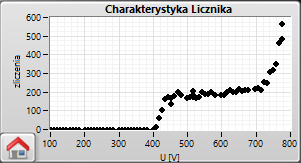
\includegraphics{Licznik.PNG}
\end{figure}\\
Do dalszych obliczeń przyjęliśmy, że najhardziej optymalne napięcie wynosi 568V, ponieważ jest to wartość najbliżej środka ze wszystkich możliwych wartości dyskretnych do wyboru.


\subsection{Pomiary}
\subsubsection{Pomiary osłabienia promieniowania dla materiału 1. }
\begin{table}[h!]
\centering
\begin{tabular}{|l|l|l|l|l|l|}
\hline
x[mm]	&	u(x)	&	N	&	U(N)	&	ln(N)	&	u(ln(N))	 \\ \hline
0	&	0.01	&	96309	&	310,3369137	&	11,47531705	&	0,08714356174	\\
5	&	0.01	&	13118	&	114,5338378	&	9,481740612	&	0,1054658676	\\
10	&	0.01	&	1696	&	41,18252056	&	7,436027816	&	0,1344804007	\\
15	&	0.01	&	258	&	16,0623784	&	5,552959585	&	0,1800841488	\\
20	&	0.01	&	35	&	5,916079783	&	3,555348061	&	0,2812664141	\\
25	&	0.01	&	8	&	2,828427125	&	2,079441542	&	0,480898347	\\
30	&	0.01	&	2	&	1,414213562	&	0,6931471806	&	1,442695041	\\
\hline
\end{tabular}
\end{table}
\subsubsection{Pomiary osłabienia promieniowania dla materiału 2. }
\begin{table}[h!]
\centering
\begin{tabular}{|l|l|l|l|l|l|}
\hline
x[mm]	&	u(x)	&	N	&	U(N)	&	ln(N)	&	u(ln(N))	\\ \hline
0	&	0.01	&	96329	&	310,3691351	&	11,47552469	&	0,08714198493	\\
5	&	0.01	&	35673	&	188,8729732	&	10,48214938	&	0,09540028136	\\
10	&	0.01	&	13305	&	115,3473017	&	9,495895183	&	0,1053086603	\\
15	&	0.01	&	4761	&	69	&	8,468213009	&	0,1180886686	\\
20	&	0.01	&	1754	&	41,88078318	&	7,469654173	&	0,1338750064	\\
25	&	0.01	&	669	&	25,86503431	&	6,50578406	&	0,1537093747	\\
30	&	0.01	&	228	&	15,09966887	&	5,429345629	&	0,1841842587	\\
\hline
\end{tabular}
\end{table}

\clearpage
\subsection{Obliczenia}
\subsubsection{Wyliczenie współczynnika osłabienia promieniowania gamma dla materiału 1.}
\begin{figure}[h!]
    \centering
    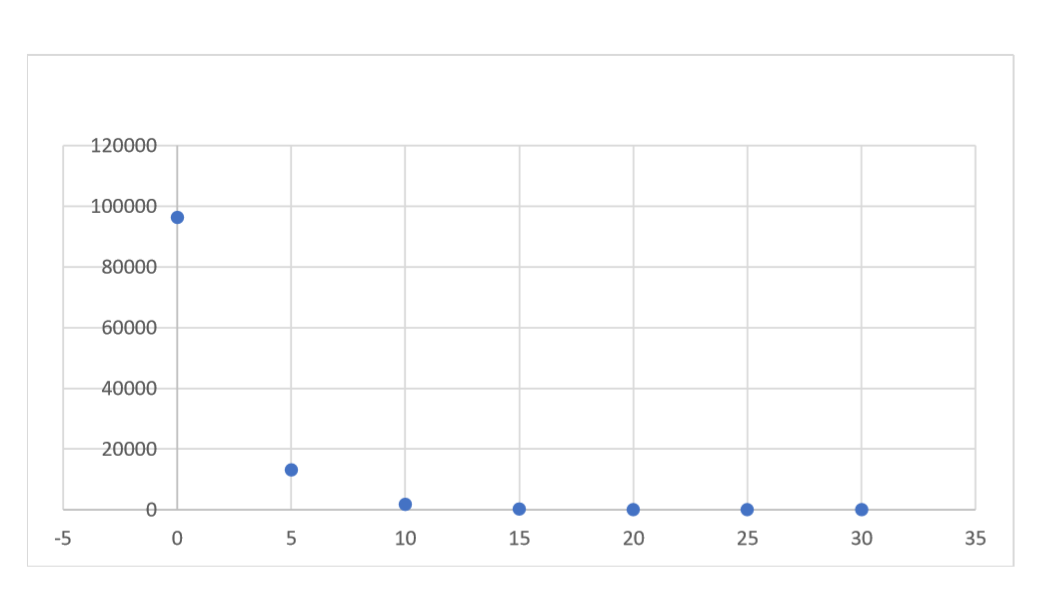
\includegraphics[scale=0.55]{1.1.png}
    \caption{Wykres liczby impulsów od grubości materiału}
\end{figure}
\begin{figure}[h!]
    \centering
    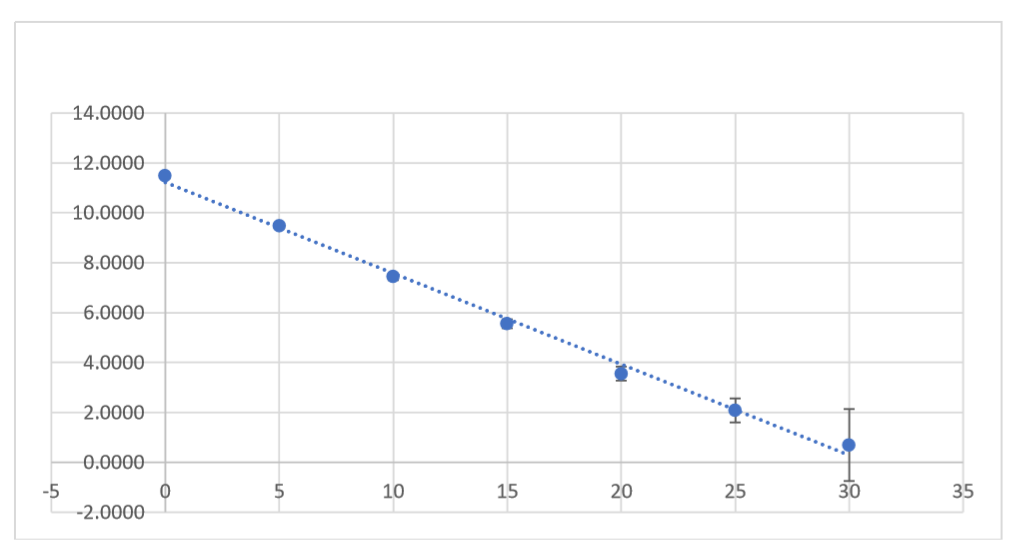
\includegraphics[scale=0.55]{1.2.png}
        \caption{Wykres logarytmu naturalnego z liczby impulsów od grubości materiału}
\end{figure}
\clearpage
\noindent Powyższe wykresy zostały wykonane za pomocą programu MS Excelktóry automatycznie liczy metodą najmniejszych kwadratów. Niepewności na osi odciętych są zaznaczone, ale są tak małe, że pokrywają się z pomiarem.\\
Drugi wykres przedstawia nam funkcję linową o poniższych parametrach
\begin{itemize}
    \item a=-0.364512768
    \item b=11.2211175
    \item u(a)=0.011201305
    \item u(b)=0.201934389
\end{itemize}
Jak wiadomo ze wzoru $\mu = -a $, a więc współczynnik osłabienia promieniowania gamma wynosi 0.364512768  dla tego materiału
\clearpage
\subsubsection{Wyliczenie współczynnika osłabienia promieniowania gamma dla materiału 2.}
\begin{figure}[h!]
    \centering
    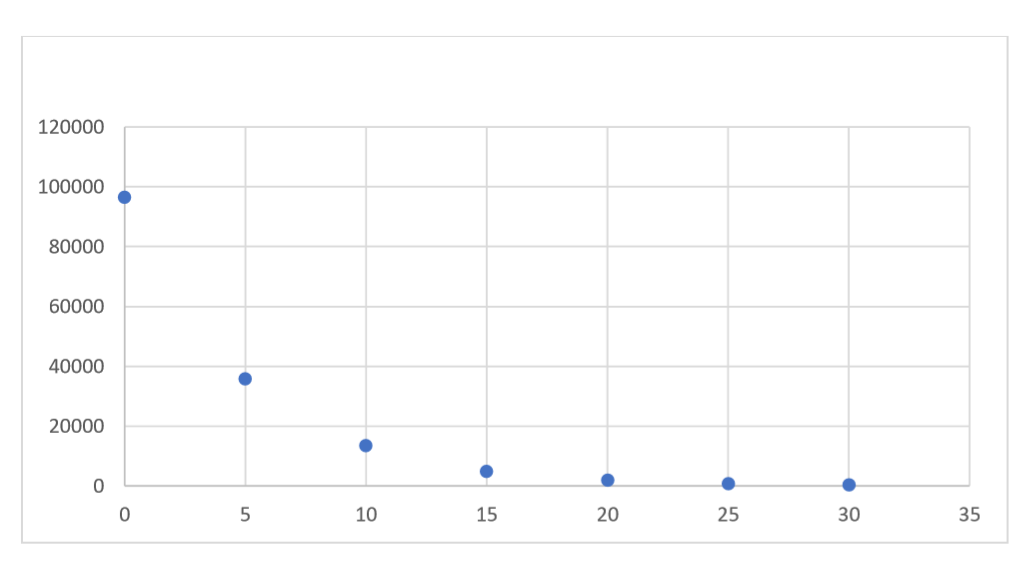
\includegraphics[scale=0.55]{2.1.png}
    \caption{Wykres liczby impulsów od grubości materiału}
\end{figure}
\begin{figure}[h!]
    \centering
    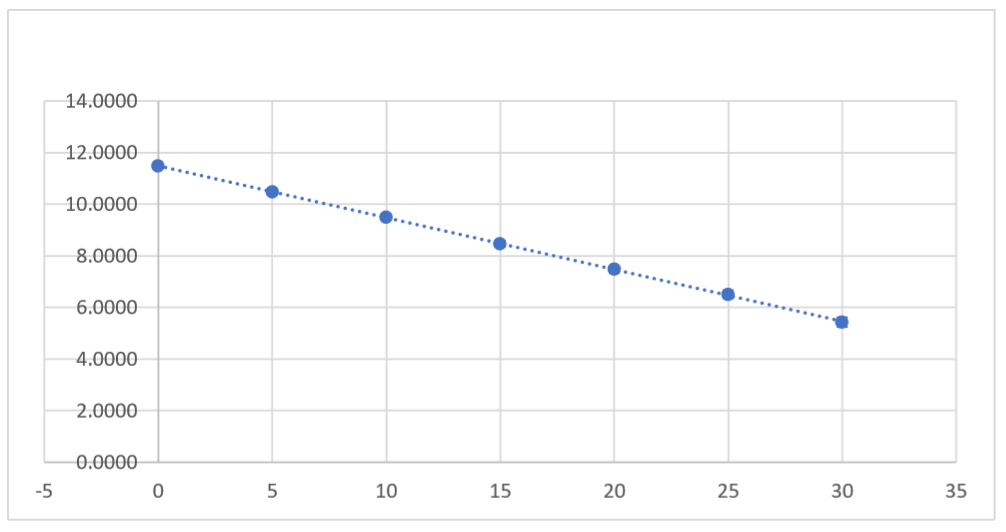
\includegraphics[scale=0.55]{2.2.png}
        \caption{Wykres logarytmu naturalnego z liczby impulsów od grubości materiału}
\end{figure}
\clearpage
\noindent Powyższe wykresy zostały wykonane za pomocą programu MS Excel, który automatycznie liczy metodą najmniejszych kwadratów. Niepewności na osi odciętych są zaznaczone, ale są tak małe, że pokrywają się z pomiarem.\\
Drugi wykres przedstawia nam funkcję linową o poniższych parametrach
\begin{itemize}
    \item a=-0.200839349
    \item b=11.48781396
    \item u(a)=0.000941293
    \item u(b)=0.016969401
\end{itemize}
Jak wiadomo ze wzoru $\mu = -a $, a więc współczynnik osłabienia promieniowania gamma wynosi 0.200839349 dla tego materiału.

\section{Wyniki}
Niestety współczynniki osłabienia zależą nie tylko od materiału, ale również energii promieniowania. W zadaniu nie została podana ani energia, ani nawet izotop z którego to promieniowanie pochodzi, czyniąc podanie materiału niemożliwym. \\
Wyliczone współczynniki wynoszą:
\begin{itemize}
    \item Dla materiału 1. --> 0.364512768(11201305) $\frac{1}{cm} $
    \item Dla materiału 2. --> 0.200839349(941293) $\frac{1}{cm} $
\end{itemize}
\section{Wnioski}
Ostatecznie wykonanie ćwiczenia pozwoliło nam na wyznaczenie współczynników osłabienia dla badanych materiałów, jednak ze względu na cyfrowy charakter wykonywanego ćwiczenia, nie jesteśmy w stanie uzyskać części danych niezbędnych do precyzyjnego wyznaczenia materiału, z którego zostały wykonane badane próbki. Jednak część doświadczalną zadania udało się przeprowadzić z sukcesem.
\end{document}

